\documentclass[italian,12pt]{article}
\usepackage{babel}
\usepackage{amssymb}
\usepackage{amsmath}
\usepackage{graphicx}

\thispagestyle{empty}
\setlength{\textwidth}{18.5cm}
\setlength{\topmargin}{-2.5cm}
\setlength{\textheight}{24.5cm}
\setlength{\oddsidemargin}{-1cm}
\setlength{\evensidemargin}{-1cm}
\begin{document}
\begin{center}{\LARGE Seconda prova parziale di Programmazione I}\\
\begin{center}
  \Large 12 giugno 2013 (tempo disponibile: 2 ore)
\end{center}
\end{center}
%\mbox{}\\
\vspace*{2ex}
\begin{center}{\Large Esercizio 1}\\
($10$ punti)
\end{center}
Le parole italiane non hanno mai pi\`u di due caratteri uguali di seguito. Si scriva una funzione
\underline{non ricorsiva}
%
\begin{verbatim}
int al_massimo_due_di_seguito(const char *s)
\end{verbatim}
%
che determina se la stringa \texttt{s} contiene al massimo due caratteri uguali di seguito.
In tal caso deve ritornare vero, altrimento falso.
%
\vspace*{2ex}
\begin{center}{\Large Esercizio 2}\\
($11$ punti)\end{center}
%
Si considerino le liste di caratteri come viste a lezione. Si definisca una funzione
%
\begin{verbatim}
struct list *construct_list_from_string(const char *s)
\end{verbatim}
%
che restituisce una lista che contiene i caratteri di \texttt{s}, nello stesso ordine.
%
\vspace*{2ex}
\begin{center}{\Large Esercizio 3}\\
($11$ punti)\end{center}
%
Si scriva una funzione \underline{ricorsiva}
%
\begin{verbatim}
struct list *doppie(struct list *this)
\end{verbatim}
%
che riceve una lista di caratteri \texttt{this}, con al massimo due caratteri uguali di seguito,
e restituisce una lista di caratteri fatta
dalle doppie contenute in \texttt{this}. In altri termini, nel risultato ci sono solo i caratteri
che sono uguali al precedente o al successivo, come nel seguente esempio:
%
\begin{center}
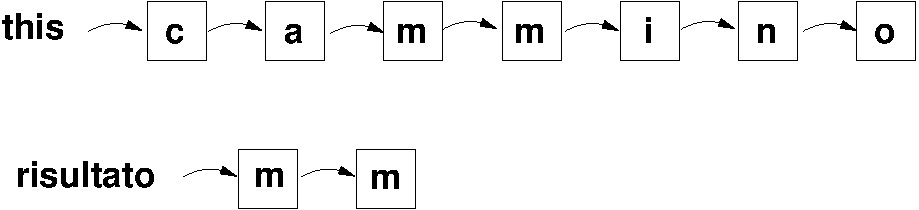
\includegraphics[scale=0.8]{doppie.pdf}
\end{center}
%
\newpage
Se tutto \`e corretto, un'esecuzione del seguente programma:
%
\begin{verbatim}
int main(void) {
  char buffer[100];
  struct list *l;

  printf("Inserisci una frase: ");
  scanf("%s", buffer);

  if (al_massimo_due_di_seguito(buffer)) {
    printf("Non ci sono piu' di due lettere uguali di seguito\n");
    l = construct_list_from_string(buffer);
    print_list(l);
    printf("\n");
    l = doppie(l);
    print_list(l);
    printf("\n");
  }
  else
    printf("Ci sono piu' di due lettere uguali di seguito\n");

  return 0;
}
\end{verbatim}
%
\`e la seguente:
%
\begin{verbatim}
Inserisci una frase: ammettere
Non ci sono piu' di due lettere uguali di seguito
[a, m, m, e, t, t, e, r, e]
[m, m, t, t]
\end{verbatim}
%
Un'altra esecuzione \`e:
%
\begin{verbatim}
Inserisci una frase: cammmino
Ci sono piu' di due lettere uguali di seguito
\end{verbatim}

\end{document}
